% ============================================================
% !TeX root = ../main.tex
%  Chapter 4 — Results and Evaluation
% ============================================================
\chapter{Results and Evaluation}
\label{ch:results}

\noindent This chapter presents the experimental evaluation of the approach
described in~\cref{ch:methodology}.

\section{Experimental Setup}
\label{sec:setup}
\noindent
The evaluation uses the final model, which was pre-trained on the synthetic
SSM meshes and then fine-tuned on the real ED and ES data, as described in~\cref{ch:methodology}. Datasets
and patient-level splits are reported in~\cref{subsec:shared-dataset-assembly}.
General reconstruction and wall-thickness evaluations use the held-out test
patients from both ACDC and M\&Ms-2. The analysis by disease group
uses a separate ACDC subset of 30 test patients, comprising 20 normal (NOR)
and 10 HCM cases. The HCM group is included so
that the model can be examined on abnormal as well as normal LV geometry. No
independent 3D ground truth is available, so the following results describe
contour fidelity and agreement between methods rather than reconstruction
accuracy. Three questions guide the evaluation: how faithfully the model
follows the observed LV contours and how far it agrees with alternative
reconstructions of them, whether it represents the ED--ES change while
maintaining a valid wall, and how closely the resulting thickness measurements
agree with those obtained from an independent method on the same input.

\subsection{Metrics}
\label{subsec:metrics}
\noindent
Reconstruction geometry is described with surface and volume measures taken
from the review of~\textcite{taha2015metrics} and from common practice in
cardiac segmentation~\parencite{bernard2018acdc} and implicit-surface
learning~\parencite{occupancynetworks2019}. They are used between a
reconstruction and the contour rings it was built from, where they show how
closely the surface follows the observations, and between two reconstructions
of the same rings, where they show how much the methods differ without
blaming either one.

The \emph{contour distance} is the gap from each observed ring point to the
nearest point of the reconstructed surface, summarised by its mean and upper
percentile; it only checks the acquired slices, not the surface between them.
The \emph{Chamfer distance}~\parencite{deepsdf2019} averages the nearest-point
gaps between two surfaces in both directions, and \emph{HD95}, the Hausdorff
distance taken at its upper percentile~\parencite{taha2015metrics}, reports
the large gaps that this average hides. Both are given in millimetres for the
endocardium and the epicardium.

The \emph{Dice similarity coefficient} (DSC)~\parencite{taha2015metrics}
compares volumes rather than surfaces: the cavity inside the endocardium and
the myocardium between the two surfaces, each filled on a shared voxel grid.
It is the shared volume relative to the total volume of both reconstructions,
rising from no overlap to complete overlap; these volumes come from the
reconstructed meshes, not from independent 3D annotations. Enclosed
\emph{volumes} are also reported in millilitres for each method separately,
the epicardial value including both cavity and wall, and the \emph{watertight
rate}, the fraction of meshes closed without holes, is a requirement for these
volumes to exist rather than a score. The average symmetric surface distance,
intersection over union, F-score and normal consistency are left out because
they repeat the Chamfer distance or the DSC, depend on a chosen tolerance, or
measure orientation rather than position.

Wall thickness is summarised by the mean, SD, and lower and upper percentiles
across the myocardial surface, in millimetres; the SD describes how much the
thickness varies over one wall and the percentiles mark its thin and thick
ends without relying on single extreme values. Between phases, the absolute
thickening $\Delta_{\text{ES}-\text{ED}}$ is the ES minus the ED thickness and
the relative thickening is that increase as a percentage of the ED value.

Agreement between wall-thickness measurements follows~\textcite{blandaltman1986}
and uses paired values, either patient means or measurements at the same
surface points. The \emph{Pearson correlation coefficient} $r$ shows whether
two methods rank the same patients or locations as thicker, not whether their
values match. The \emph{mean absolute error} (MAE) is the average size of the
difference in millimetres, and the \emph{root-mean-square error} (RMSE) gives
more weight to large differences. The Bland--Altman \emph{bias} is the mean
signed difference, showing whether one method reads consistently higher, and
the \emph{limits of agreement} (LoA) give the range expected to contain most
individual differences. The two-way \emph{intraclass correlation coefficient}
(ICC) rates agreement against the spread of the paired values and, unlike
$r$, penalises a constant offset; it is read against the thresholds
of~\textcite{koo2016icc}.

\subsection{Methods Used for Comparison}
\label{subsec:baselines}
\noindent
The reconstruction is compared with two
alternative reconstructions of the same input contour rings: a
radial-basis-function implicit fit, which interpolates the rings through a
smooth field, and a fit of the public SSM, which
keeps the reconstructed shape within the variation represented by the
population model. These methods make different assumptions about the shape
between slices, so differences between their results show how strongly those
assumptions affect the reconstructed geometry. Both
use the same rings as the model and undergo the same mesh repair and
measurement steps, as described in~\cref{subsec:inference-offset-extraction}, so their numbers are directly
comparable. They are evaluated only at ED: the public SSM is distributed with
ED modes only.

The RBF fit is used for comparison, not as ground truth. It belongs
to the same family as the surfaces fitted to the contours for training, so close
agreement with the model is partly expected and is not independent
confirmation. By contrast, the SSM fit is independent of the training targets, but
some patients have shapes outside the variation represented by its training
population. Wall
thickness is compared between
the model, the RBF fit, and the SSM fit with the four algorithms selected in~\cref{subsec:thickness-methods}: the Laplace field method, the Yezzi--Prince
method, the SDF cone-ray method, and the EDT boundary sum. Because the SAX stacks are sparse relative to their in-plane
resolution, all three reconstruction methods must infer the through-plane
geometry, and their absolute millimetre values should be read with care.

\section{Training}
\label{sec:training}
\noindent
Training proceeds in two stages. The first pre-trains
the signed-distance decoder for roughly 200 epochs on the synthetic SSM
meshes. This stage provides a geometric prior, and its checkpoint initialises
the second stage. The reported model is then fine-tuned on the real
ED and ES data described in~\cref{ch:methodology}. The
available training history records the fine-tuning stage; no numerical claim is
made about the pre-training loss because its per-epoch log was not retained.

Fine-tuning runs for 776 epochs with the AdamW optimiser (learning rate
$2\times10^{-5}$, weight decay $5\times10^{-4}$) under a cosine-annealing
schedule with warm restarts, mixed-precision arithmetic, and an effective batch
size of 32. The composite objective is the five-term loss of~\cref{eq:training-objective}, combining surface, dense SDF, Eikonal,
off-surface, and wall-thickness supervision. \Cref{fig:training-curves} plots
the total loss and its principal components together with two optimisation
diagnostics. The total
training loss decreases from 10.07 at the first fine-tuning epoch to 0.91,
and the validation loss settles at 0.70, with the best checkpoint selected at
epoch 695 before mild over-fitting appears. The surface and Eikonal terms fall
by more than an order of magnitude, indicating successful optimisation of the
surface-fitting and Eikonal objectives. Consistently, the mean gradient norm
$\lVert\nabla f\rVert$ stabilises at 0.996, close to the unit value encouraged
by the Eikonal term.

\begin{figure}[H]
  \centering
  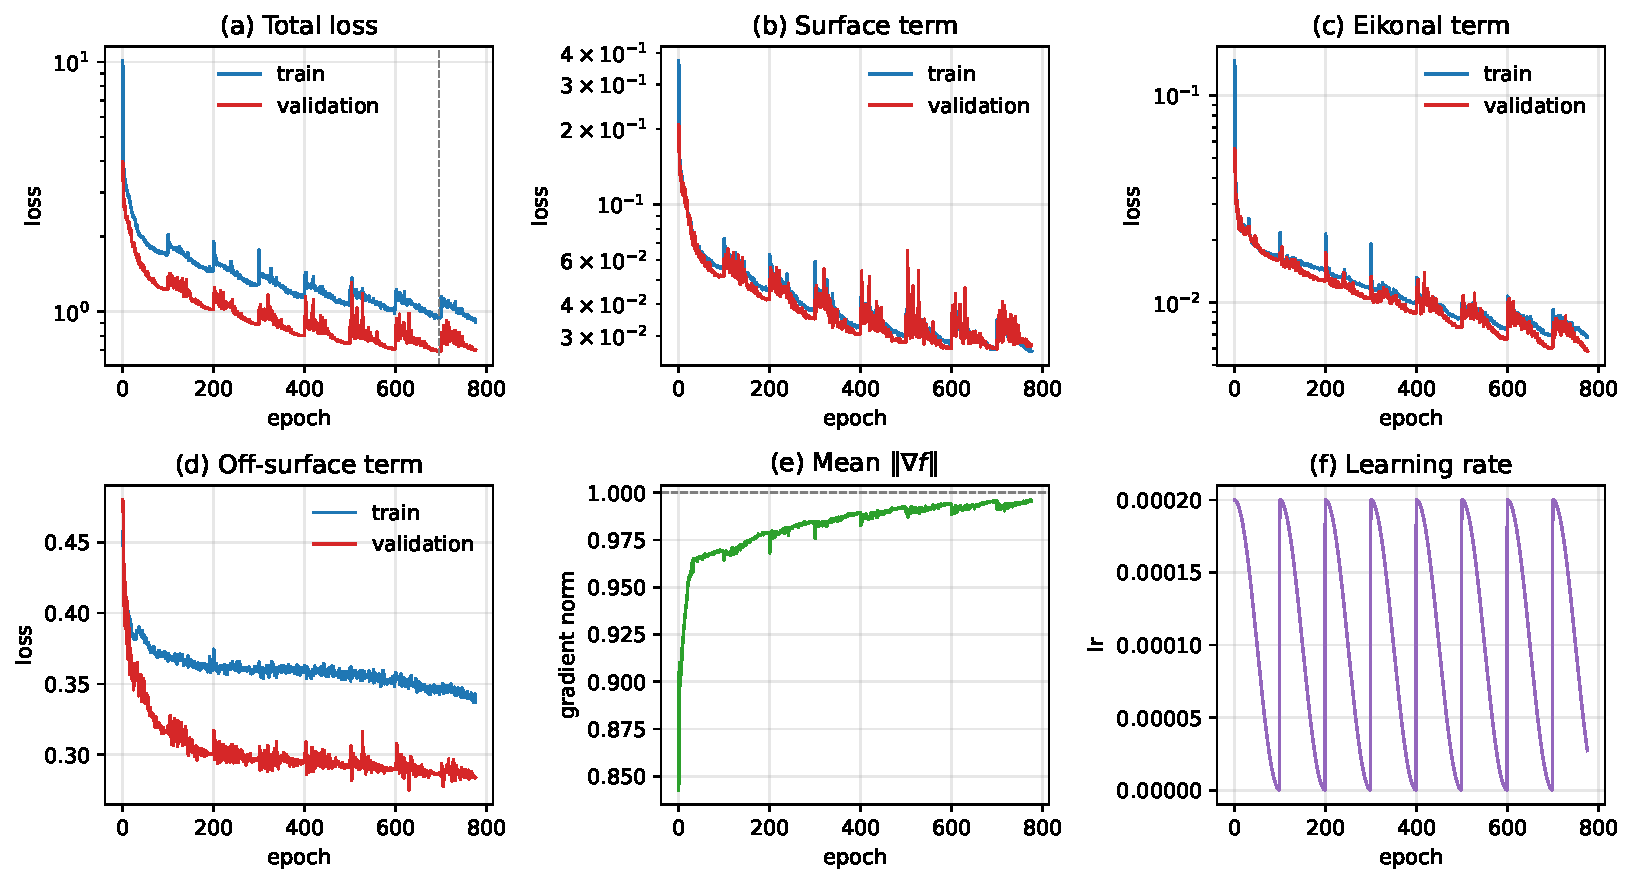
\includegraphics[width=\textwidth]{training_curves}
  \caption[Training history]{Training history. (a)--(d) Total loss and its
    surface, Eikonal, and off-surface components for the training and
    validation splits; the dashed line marks the best epoch. (e)--(f) Mean
    gradient norm (target one) and cosine-annealing learning rate. Synthetic
    pre-training is not shown.}
  \label{fig:training-curves}
\end{figure}

\section{Results}
\label{sec:results}
\noindent
Three analyses cover reconstruction consistency, wall-thickness measurement,
and regional analysis with the AHA 17-segment model.

\subsection{Reconstruction Consistency}
\label{subsec:reconstruction-quality}
\noindent
Contour fidelity measures how closely each surface follows its input rings, and
pairwise agreement measures how much the three reconstructions differ from one
another. All values below are at ED and cover the held-out ACDC and M\&Ms-2
test cohort. Every surface from every method is watertight after the shared
repair stage.

\vspace{-2mm}

\begin{figure}[H]
  \centering
  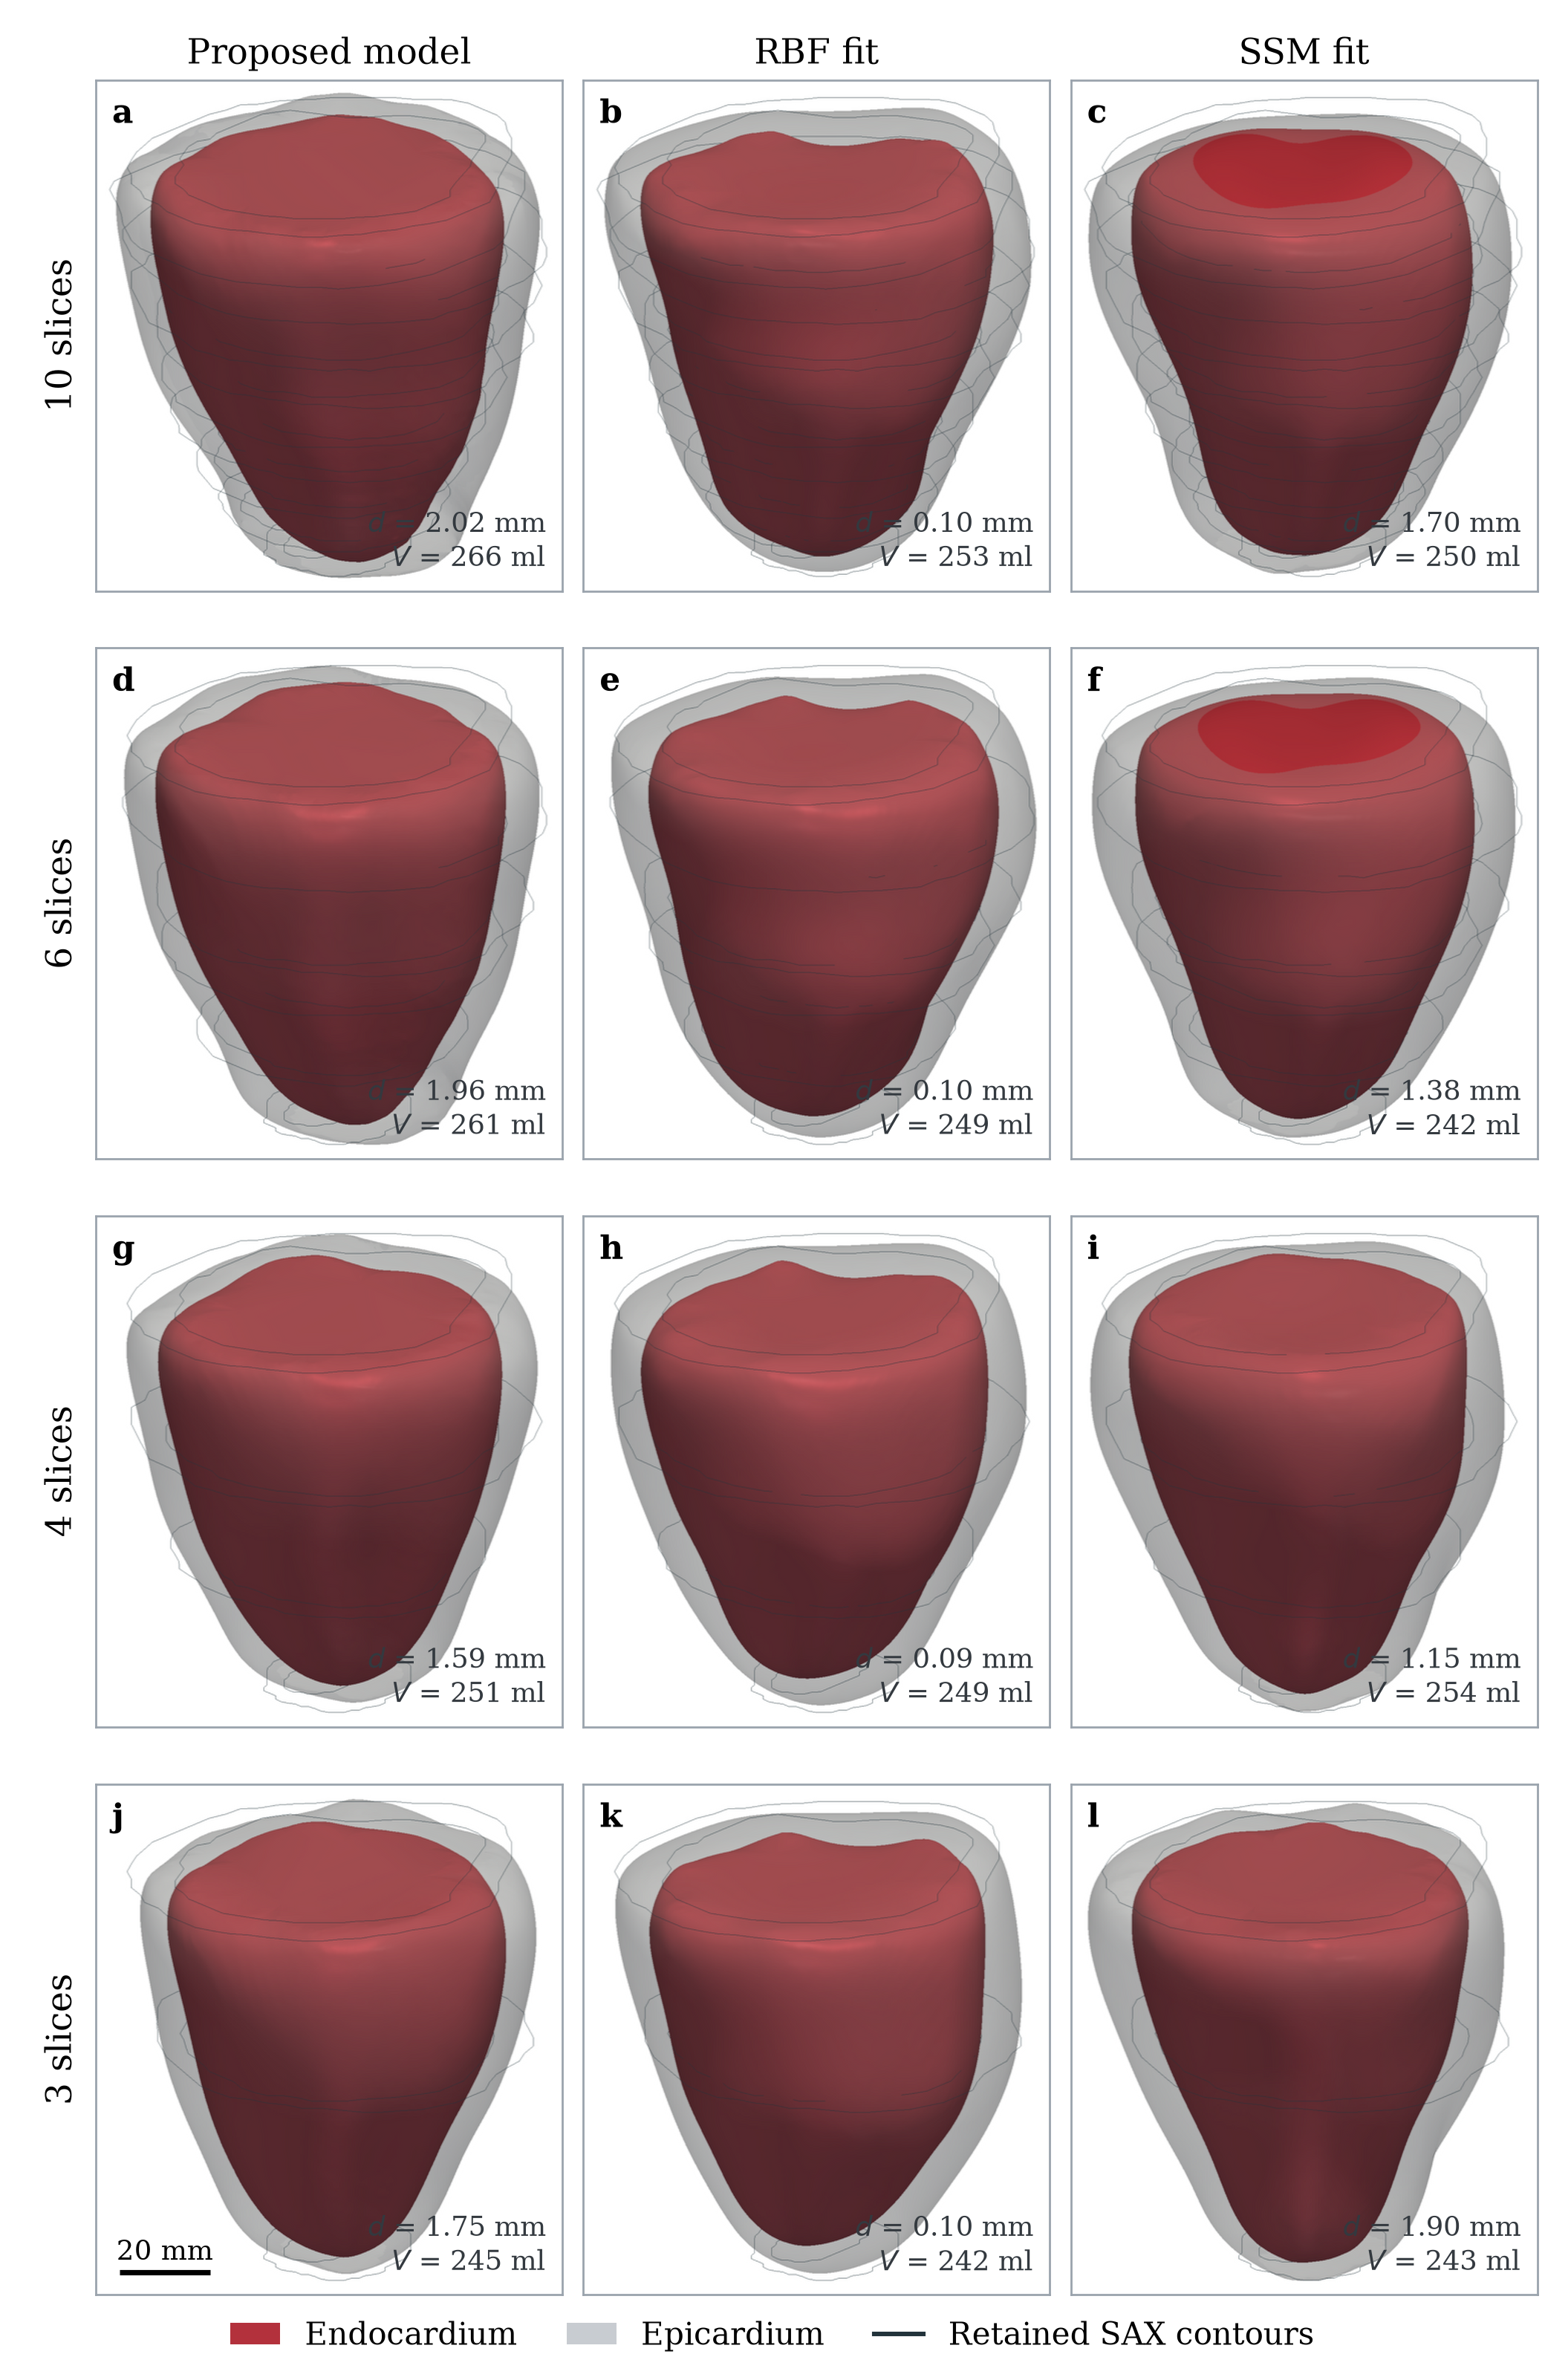
\includegraphics[width=0.75\textwidth]{results_slice_ablation}
  \caption[LV surfaces recovered from progressively sparser SAX stacks]  {Left-ventricular surfaces of one ACDC case
      reconstructed from an ED SAX stack with ten, six, four, and three retained
      slices (rows) by the proposed model, RBF fit, and SSM fit (columns). Red:
      endocardium; grey: epicardium; dark rings: input contours.}
  \label{fig:slice-ablation}
\end{figure}

\vspace{-2mm}

\Cref{fig:slice-ablation} shows one case reconstructed by the three methods. In
the complete ten-slice row, the three surfaces share the same overall
ventricular shape. The reduced-slice rows are analysed in~\cref{subsec:slice-sensitivity}.

\Cref{tab:contour-fidelity} reports the distance from each input contour ring to
the reconstructed surface and the enclosed volumes, the endocardial value being
the cavity alone and the epicardial value the cavity together with the wall.

\begin{table}[H]
  \centering
  \caption[Fidelity of each reconstruction to its input contours]    {Distance from the input SAX contour rings to
      each reconstructed surface, and enclosed volumes, at ED over the held-out
      test cohort (mean~\textpm{} SD of per-patient values; $p_{95}$: mean
      per-patient 95th percentile). Bold marks the lowest distance.}
  \label{tab:contour-fidelity}
  \thesistablestyle
  \begin{tabular*}{\textwidth}{@{\extracolsep{\fill}}l l c c c@{}}
    \toprule
    \textbf{Method} & \textbf{Surface} & \textbf{Contour distance (mm)}
      & \textbf{$p_{95}$ (mm)} & \textbf{Volume (ml)} \\
    \midrule
    Proposed model  & Endocardium & 1.50~\textpm{} 0.23 & 3.56 & 119.3~\textpm{} 31.3 \\
                    & Epicardium  & 1.96~\textpm{} 0.28 & 5.23 & 255.3~\textpm{} 76.7 \\
    \addlinespace
    RBF fit         & Endocardium & \textbf{0.13~\textpm{} 0.01} & \textbf{0.30} & 118.6~\textpm{} 30.2 \\
                    & Epicardium  & \textbf{0.11~\textpm{} 0.01} & \textbf{0.26} & 233.5~\textpm{} 71.4 \\
    \addlinespace
    SSM fit         & Endocardium & 1.82~\textpm{} 0.67 & 5.51 & 126.9~\textpm{} 32.2 \\
                    & Epicardium  & 1.91~\textpm{} 0.76 & 6.23 & 215.2~\textpm{} 56.3 \\
    \bottomrule
  \end{tabular*}
\end{table}

The RBF fit follows the rings almost exactly, at 0.13~mm on the endocardium
and 0.11~mm on the epicardium, because it passes through the contour points
by construction. The model lies 1.50 and 1.96~mm from the same rings,
which is close to the in-plane pixel size of 1.37 to 1.88~mm. The SSM fit
has similar mean distances, 1.82 and 1.91~mm, but a wider spread between
patients: its per-patient endocardial distance ranges from 0.92 to
3.44~mm, against 1.20 to 2.14~mm for the model.

In the 30-patient ACDC pathology subset, the mean contour distance of the SSM
fit is 1.42~mm for normal cases and 2.63~mm for HCM cases. The
corresponding model distances are 1.45 and 1.60~mm.

Cavity volumes are similar for the model, the RBF fit and the SSM fit, at
119, 119 and 127~ml, respectively. Myocardial volumes, obtained as the
epicardial minus the cavity volume, differ more, at 136, 115 and 88~ml.

\Cref{tab:reconstruction-agreement} compares the three reconstructions with one
another, by the distance between their boundaries and by the overlap of the
cavity and wall that those boundaries enclose.

\begin{table}[H]
  \centering
  \caption[Pairwise agreement between the three reconstructions]    {Pairwise agreement between the three
      reconstructions of the same ED contour rings over the held-out test cohort
      (mean~\textpm{} SD of per-patient values). Entries are symmetric disagreements,
      not errors against a reference. Bold marks the closest pair.}
  \label{tab:reconstruction-agreement}
  \thesistablestyle
  \begin{tabular*}{\textwidth}{@{\extracolsep{\fill}}l l c c@{}}
    \toprule
    \textbf{Pair} & \textbf{Metric} & \textbf{Endocardium/cavity}
      & \textbf{Epicardium/myocardium} \\
    \midrule
    Model vs.\ RBF fit   & Chamfer (mm) & \textbf{1.57~\textpm{} 0.18} & \textbf{1.90~\textpm{} 0.24} \\
                          & HD95 (mm)     & \textbf{4.24~\textpm{} 0.86} & \textbf{6.07~\textpm{} 0.94} \\
                          & DSC           & \textbf{0.91~\textpm{} 0.02} & \textbf{0.77~\textpm{} 0.05} \\
    \addlinespace
    Model vs.\ SSM fit   & Chamfer (mm) & 2.08~\textpm{} 0.51 & 2.59~\textpm{} 0.73 \\
                          & HD95 (mm)     & 5.88~\textpm{} 1.91 & 6.72~\textpm{} 2.32 \\
                          & DSC           & 0.88~\textpm{} 0.03 & 0.69~\textpm{} 0.04 \\
    \addlinespace
    RBF fit vs.\ SSM fit & Chamfer (mm) & 2.01~\textpm{} 0.67 & 2.05~\textpm{} 0.64 \\
                          & HD95 (mm)     & 5.88~\textpm{} 2.95 & 6.62~\textpm{} 2.67 \\
                          & DSC           & 0.89~\textpm{} 0.04 & 0.76~\textpm{} 0.06 \\
    \bottomrule
  \end{tabular*}
\end{table}

The model and the RBF fit form the closest pair on every metric and surface,
with Chamfer distances of 1.57~mm on the endocardium and 1.90~mm on the
epicardium and a myocardial DSC of 0.77. Both pairs involving the SSM fit are
further apart, at 2.08 and 2.01~mm on the endocardium.

Across the three pairs, the endocardial Chamfer distance ranges from 1.6 to
2.1~mm. Cavity DSC is uniformly high, at 0.88 to 0.91, whereas
myocardial DSC is lower, at 0.69 to 0.77, and falls to 0.58 for the
worst patient in a comparison involving the SSM fit.

\subsection{Slice Sensitivity}
\label{subsec:slice-sensitivity}
\noindent
Each patient's complete ED stack is reduced to six, four and three slices. The
most basal and most apical slices are always kept, so the base-to-apex extent
stays the same and only the number of slices within it changes. Because the
acquired stacks differ in length, a patient contributes to a given level only
when its complete stack has more slices than that level. The lower rows of~\cref{fig:slice-ablation} show the effect on one case.

\begin{table}[H]
  \centering
  \caption[Effect of removing slices from each reconstruction]{Deviation of
  each method's reduced-slice reconstruction from its complete-stack
  reconstruction at ED on the held-out test cohort. Bold marks the smallest
  deviation at each slice level.}
  \label{tab:slice-degradation}
  \thesistablestyle
  \begin{tabular*}{\textwidth}{@{\extracolsep{\fill}}l c c c c c c@{}}
    \toprule
    & & \multicolumn{2}{c}{\textbf{Chamfer (mm)}}
      & \multicolumn{2}{c}{\textbf{DSC}} & \\
    \cmidrule(lr){3-4} \cmidrule(lr){5-6}
    \textbf{Method} & \textbf{Slices} & \textbf{Endo.} & \textbf{Epi.}
      & \textbf{Cavity} & \textbf{Myoc.}
      & \textbf{$\Delta V_{\text{myo}}$ (\%)} \\
    \midrule
    Proposed model & 6 & \textbf{0.79} & 0.87 & \textbf{0.971} & \textbf{0.891} & \textminus{}0.4 \\
                   & 4 & 1.27 & 1.48 & 0.953 & 0.819 & \textminus{}2.1 \\
                   & 3 & 1.83 & 2.17 & 0.934 & 0.782 & \textminus{}3.8 \\
    \addlinespace
    RBF fit        & 6 & 0.83 & \textbf{0.83} & 0.968 & 0.887 & \textbf{0.0} \\
                   & 4 & \textbf{1.15} & \textbf{0.88} & \textbf{0.959} & \textbf{0.858} & \textbf{\textminus{}1.8} \\
                   & 3 & \textbf{1.45} & \textbf{1.32} & \textbf{0.947} & \textbf{0.805} & \textminus{}6.2 \\
    \addlinespace
    SSM fit        & 6 & 0.89 & 0.95 & 0.968 & 0.883 & \textminus{}1.8 \\
                   & 4 & 1.46 & 1.39 & 0.942 & 0.812 & \textminus{}3.8 \\
    & 3 & 1.94 & 1.92 & 0.921 & 0.775 & \textbf{+2.6} \\
    \bottomrule
  \end{tabular*}
\end{table}

\Cref{tab:slice-degradation} compares each reduced-stack reconstruction with
the one the same method produces from the complete stack, so the values show
the effect of removing slices rather than the differences between methods;
$\Delta V_{\text{myo}}$ is the change in wall volume relative to that
complete-stack result. All three methods still produce closed surfaces from
three slices.

With six slices, the reconstructions change very little: surface distances
stay below 1~mm and myocardial DSC is close to 0.89 for every method. With
fewer slices, the RBF fit changes least, while the model and the SSM fit
change by similar amounts. The difference is clearest on the epicardium, where
the Chamfer distance at three slices reaches 2.17~mm for the model,
1.92~mm for the SSM fit and 1.32~mm for the RBF fit. Cavity DSC stays
above 0.92 throughout, and myocardial DSC at three slices lies between
0.775 and 0.805.

Myocardial volume changes by only a few percent. At three slices, the model
and the RBF fit lose 3.8\% and 6.2\%, whereas the SSM fit gains 2.6\%
after losing volume with six and four slices, so its small change at that
level does not mean that it follows the complete-stack volume more closely.

\subsection{Wall-Thickness Measurement}
\label{subsec:wall-thickness-results}
\noindent
The four selected methods are applied to the proposed reconstruction, the RBF
fit, and the SSM fit for every patient at ED.
\Cref{tab:wall-thickness-results} reports, for each method and reconstruction,
the cohort average of the per-patient mean, SD, and 5th and 95th
percentiles, the SD describing variation across each patient's wall rather
than between patients.

\begin{table}[H]
  \centering
  \caption[ED wall-thickness statistics]{Wall-thickness statistics at ED over the held-out ACDC and
    M\&Ms-2 test cohort. Each entry is the cohort average of the corresponding
    per-patient statistic, in millimetres.}
  \label{tab:wall-thickness-results}
  \thesistablestyle
  \begin{tabular*}{\textwidth}{@{\extracolsep{\fill}}l l c c c c@{}}
    \toprule
    \textbf{Method} & \textbf{Geometry} & \textbf{Mean (mm)}
      & \textbf{SD (mm)} & \textbf{$p_{5}$ (mm)} & \textbf{$p_{95}$ (mm)} \\
    \midrule
      Laplace field    & Model &  9.18 & 2.14 & 4.75 & 12.20 \\
                       & RBF fit &  8.36 & 2.21 & 5.03 & 12.29 \\
                       & SSM fit &  6.48 & 1.38 & 3.87 &  8.43 \\
      \addlinespace
      Yezzi--Prince    & Model & 10.01 & 1.64 & 7.41 & 12.74 \\
               & RBF fit &  8.86 & 2.15 & 5.57 & 12.71 \\
               & SSM fit &  7.10 & 1.23 & 4.75 &  8.88 \\
      \addlinespace
      SDF cone rays    & Model & 12.47 & 4.87 & 8.01 & 20.68 \\
                       & RBF fit &  9.38 & 2.49 & 5.63 & 13.80 \\
                       & SSM fit &  7.11 & 1.50 & 4.12 &  9.13 \\
      \addlinespace
      EDT boundary sum & Model &  9.55 & 1.66 & 6.62 & 12.17 \\
                       & RBF fit &  8.51 & 2.00 & 5.42 & 12.05 \\
                       & SSM fit &  7.02 & 1.22 & 4.65 &  8.77 \\
    \bottomrule
  \end{tabular*}
\end{table}

The three non-ray methods agree closely on each reconstruction, with mean
thicknesses of 9.18 to 10.01~mm on the proposed reconstruction, 8.36 to
8.86~mm on the RBF fit and 6.48 to 7.10~mm on the SSM fit. The SDF
cone-ray method stands apart on the first two, at 12.47 and 9.38~mm, and
also spreads more widely: on the proposed reconstruction, its per-patient SD is
4.87~mm, against 1.64 to 2.14~mm for the other methods.

\Cref{tab:wall-thickness-geometry-agreement} compares patient-level mean
thickness on the proposed reconstruction with the two fitting baselines, with
the measurement algorithm held fixed so that differences reflect the geometry
alone.

\begin{table}[H]
  \centering
  \caption[Wall-thickness agreement between reconstructions]  {Patient-level agreement between wall
      thickness on the proposed reconstruction and on each fitting baseline at
      ED. Bias is the model value minus the baseline value. Bold marks the
      closest agreement in each column.}
  \label{tab:wall-thickness-geometry-agreement}
  \thesistablestyle
  \begin{tabular*}{\textwidth}{@{\extracolsep{\fill}}l c c c c c c@{}}
    \toprule
    & \multicolumn{3}{c}{\textbf{Model vs. RBF fit}}
      & \multicolumn{3}{c}{\textbf{Model vs. SSM fit}} \\
    \cmidrule(lr){2-4} \cmidrule(lr){5-7}
    \textbf{Method} & \textbf{Bias (mm)} & \textbf{RMSE (mm)} & \textbf{$r$}
      & \textbf{Bias (mm)} & \textbf{RMSE (mm)} & \textbf{$r$} \\
    \midrule
    Laplace field    & \textbf{+0.82} & \textbf{0.86} & \textbf{0.99} & +2.70 & 3.13 & 0.72 \\
    Yezzi--Prince    & +1.16 & 1.23 & \textbf{0.99} & +2.91 & 3.49 & \textbf{0.77} \\
    SDF cone rays    & +3.10 & 3.81 & 0.95 & +5.36 & 6.64 & 0.67 \\
    EDT boundary sum & +1.03 & 1.10 & \textbf{0.99} & \textbf{+2.53} & \textbf{3.04} & \textbf{0.77} \\
    \bottomrule
  \end{tabular*}
\end{table}

With the same measurement method on each geometry, the RBF fit is thinner than
the model by 0.82~mm for the Laplace field, 1.16~mm for Yezzi--Prince,
3.10~mm for SDF cone rays, and 1.03~mm for the EDT boundary sum. The SSM
fit is thinner by 2.70, 2.91, 5.36, and 2.53~mm, respectively.
Per-patient means are strongly correlated between the model and the RBF fit
($r=0.99$, 0.99, 0.95, and 0.99) and less strongly between the model and
the SSM fit ($r=0.72$, 0.77, 0.67, and 0.77).

\Cref{tab:wall-thickness-agreement} compares the three other methods with the
Laplace field at the same surface points on the proposed reconstruction, so
that only the measurement algorithm changes.

\begin{table}[H]
  \centering
  \caption[Wall-thickness-method agreement with Laplace]{Agreement of each
  wall-thickness method with the Laplace field over the myocardial surface
  points of the held-out test cohort. Bias is the method value minus the
  Laplace-field value. The Laplace field is the reference for comparison,
  not ground truth.}
  \label{tab:wall-thickness-agreement}
  \thesistablestyle
  \begin{tabular*}{\textwidth}{@{\extracolsep{\fill}}l c c c c c@{}}
    \toprule
    \textbf{Method} & \textbf{$r$} & \textbf{MAE (mm)}
      & \textbf{RMSE (mm)} & \textbf{Bias (95\% LoA) (mm)} & \textbf{ICC} \\
    \midrule
    Yezzi--Prince    & \textbf{0.80} & 0.89 & 2.14 & +0.83 (\textpm{}3.86) & \textbf{0.77} \\
    SDF cone rays    & 0.44 & 3.38 & 7.29 & +3.31 (\textpm{}12.74) & 0.28 \\
    \addlinespace
    EDT boundary sum & 0.78 & \textbf{0.81} & \textbf{2.07} & \textbf{+0.37} (\textpm{}3.99) & \textbf{0.77} \\
    \bottomrule
  \end{tabular*}
\end{table}

The EDT boundary sum differs from the Laplace field by 0.81~mm on average,
with a bias of +0.37~mm, and Yezzi--Prince by 0.89~mm, with a bias of
+0.83~mm; both reach $\text{ICC} = 0.77$, which corresponds to moderate to
good agreement under the thresholds of~\textcite{koo2016icc}. The cone-ray
method differs by 3.38~mm on average, with a bias of +3.31~mm, LoA of
\textpm{}12.74~mm and $\text{ICC} = 0.28$, which corresponds to poor agreement.

\begin{figure}[H]
  \centering
  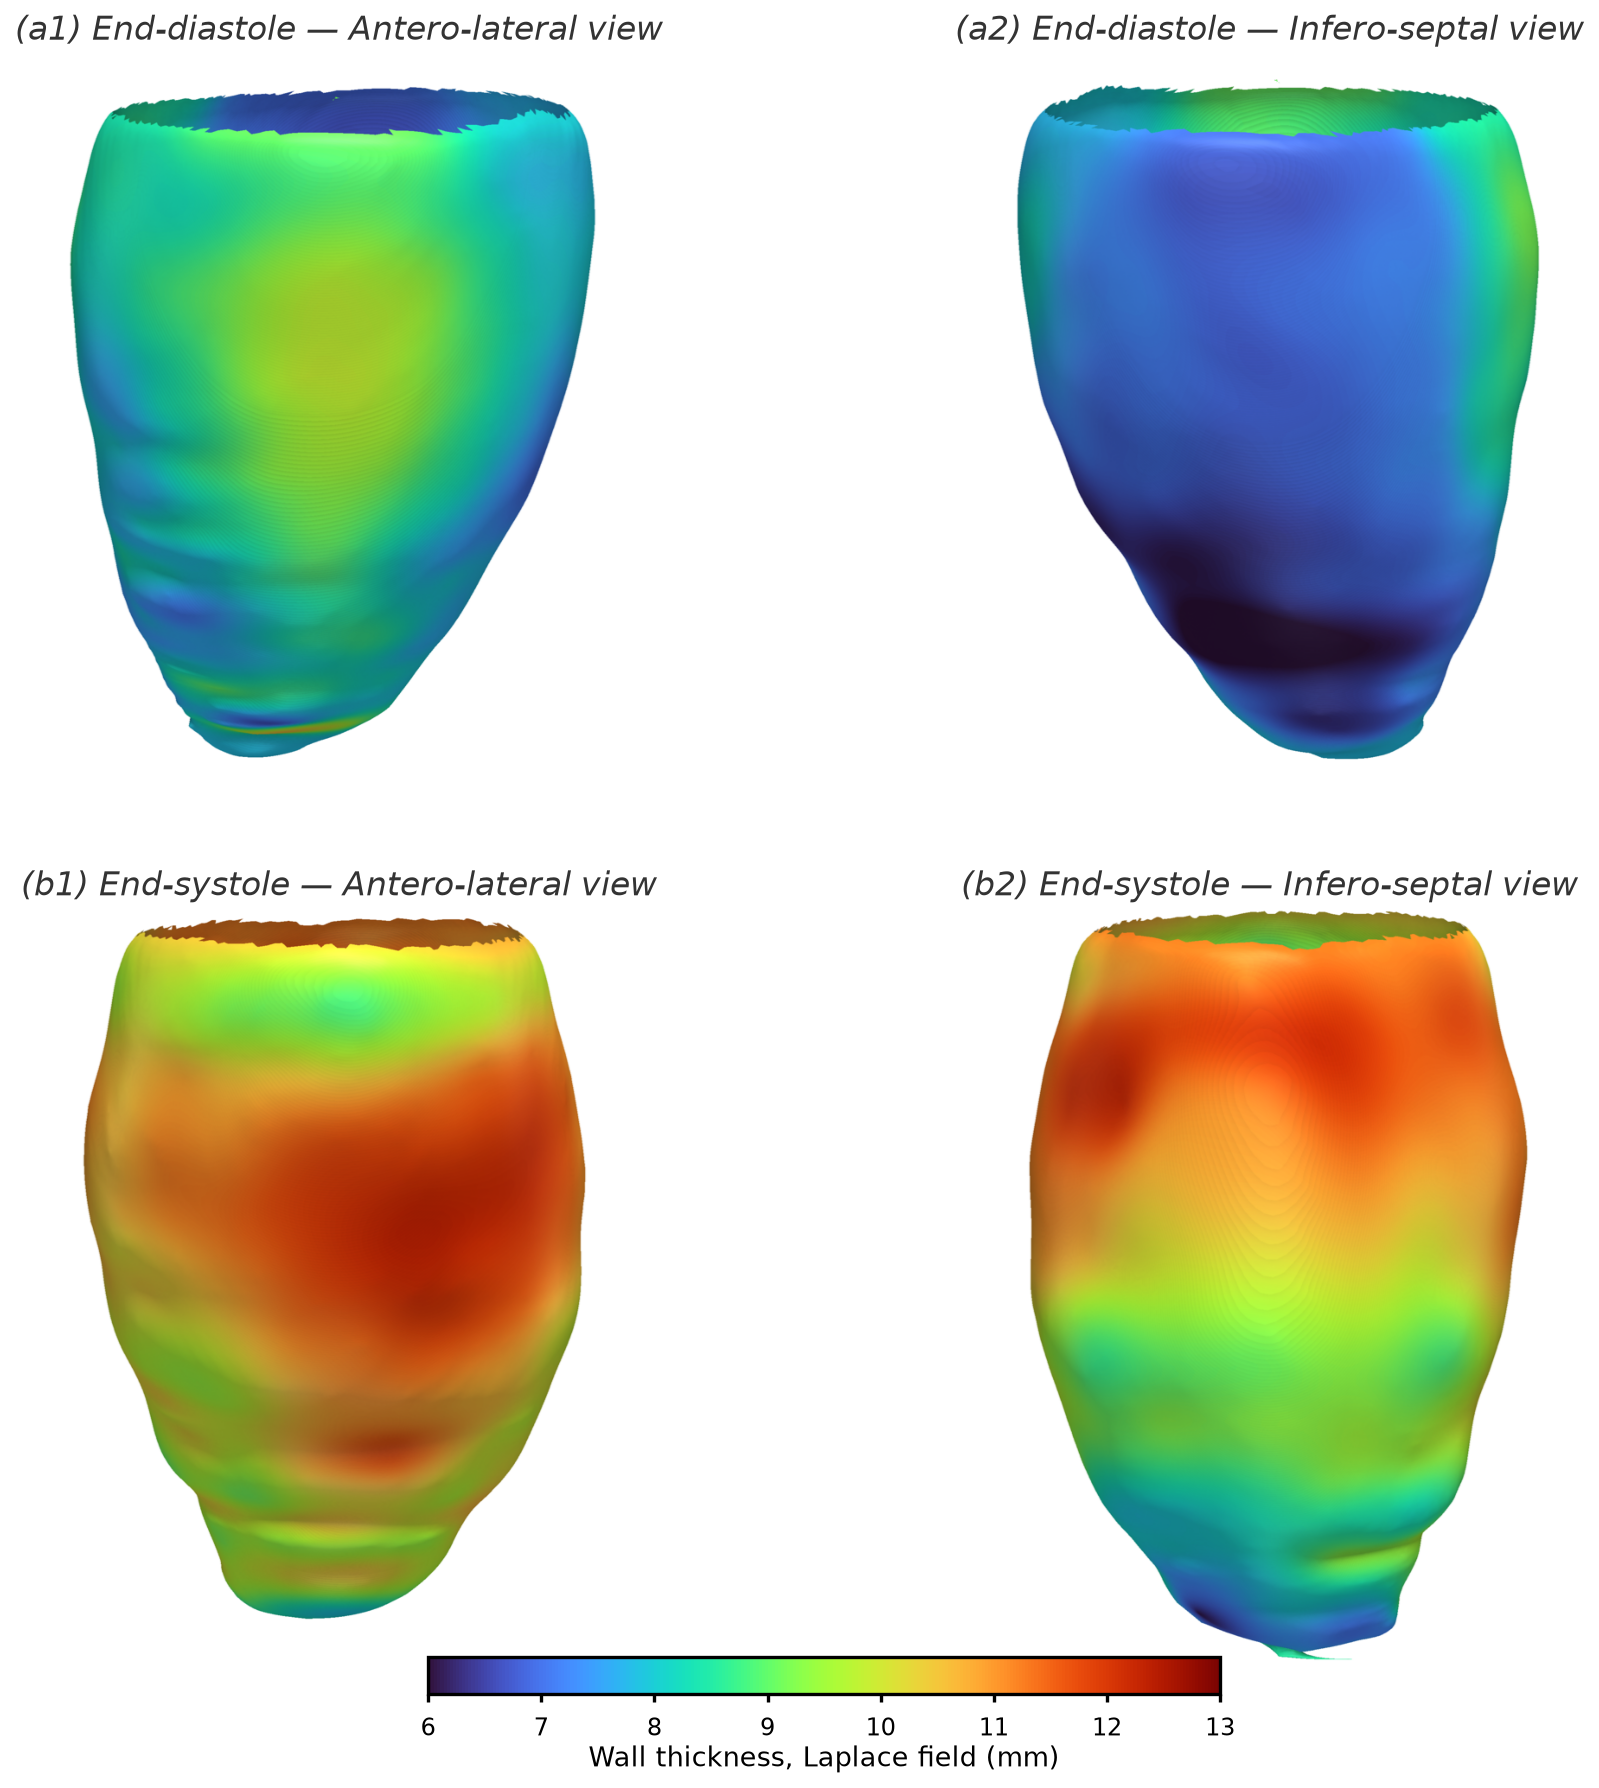
\includegraphics[width=0.78\textwidth]{results_recon_thickness_3d}
  \caption[Predicted wall-thickness map]{Predicted wall thickness on the
    reconstructed surface of one ACDC case at ED (top) and ES (bottom), shown
    from two viewpoints on a shared colour scale. Values are scaled to the input
    segmentation.}
  \label{fig:recon-thickness-3d}
\end{figure}

\Cref{fig:recon-thickness-3d} shows the predicted wall thickness as a heatmap
on the reconstructed surface. The values are scaled to the input segmentation,
so the map shows where the wall is thicker or thinner rather than its absolute
thickness. The circumferential bands follow the spacing of the SAX slices.

\subsection{Regional Analysis over the AHA 17-Segment Model}
\label{subsec:aha17-results}
\noindent
To place the measurements anatomically, the reconstructed surface is divided
into the standard AHA segments~\parencite{cerqueira2002segmentation} described
in~\cref{subsec:aha17-mapping}: basal, mid-cavity and apical sectors oriented
from the septum, plus the apical cap. Each mesh point falls into one segment
and the thickness values within it are averaged, so the surface map becomes
one mean per region that refers to the same part of the ventricle in every
patient and phase. These means are Laplace-field
thickness~\parencite{jones2000laplace} measured directly on the
meshes, not the segmentation-scaled values of~\cref{fig:recon-thickness-3d}.

\begin{figure}[H]
  \centering
  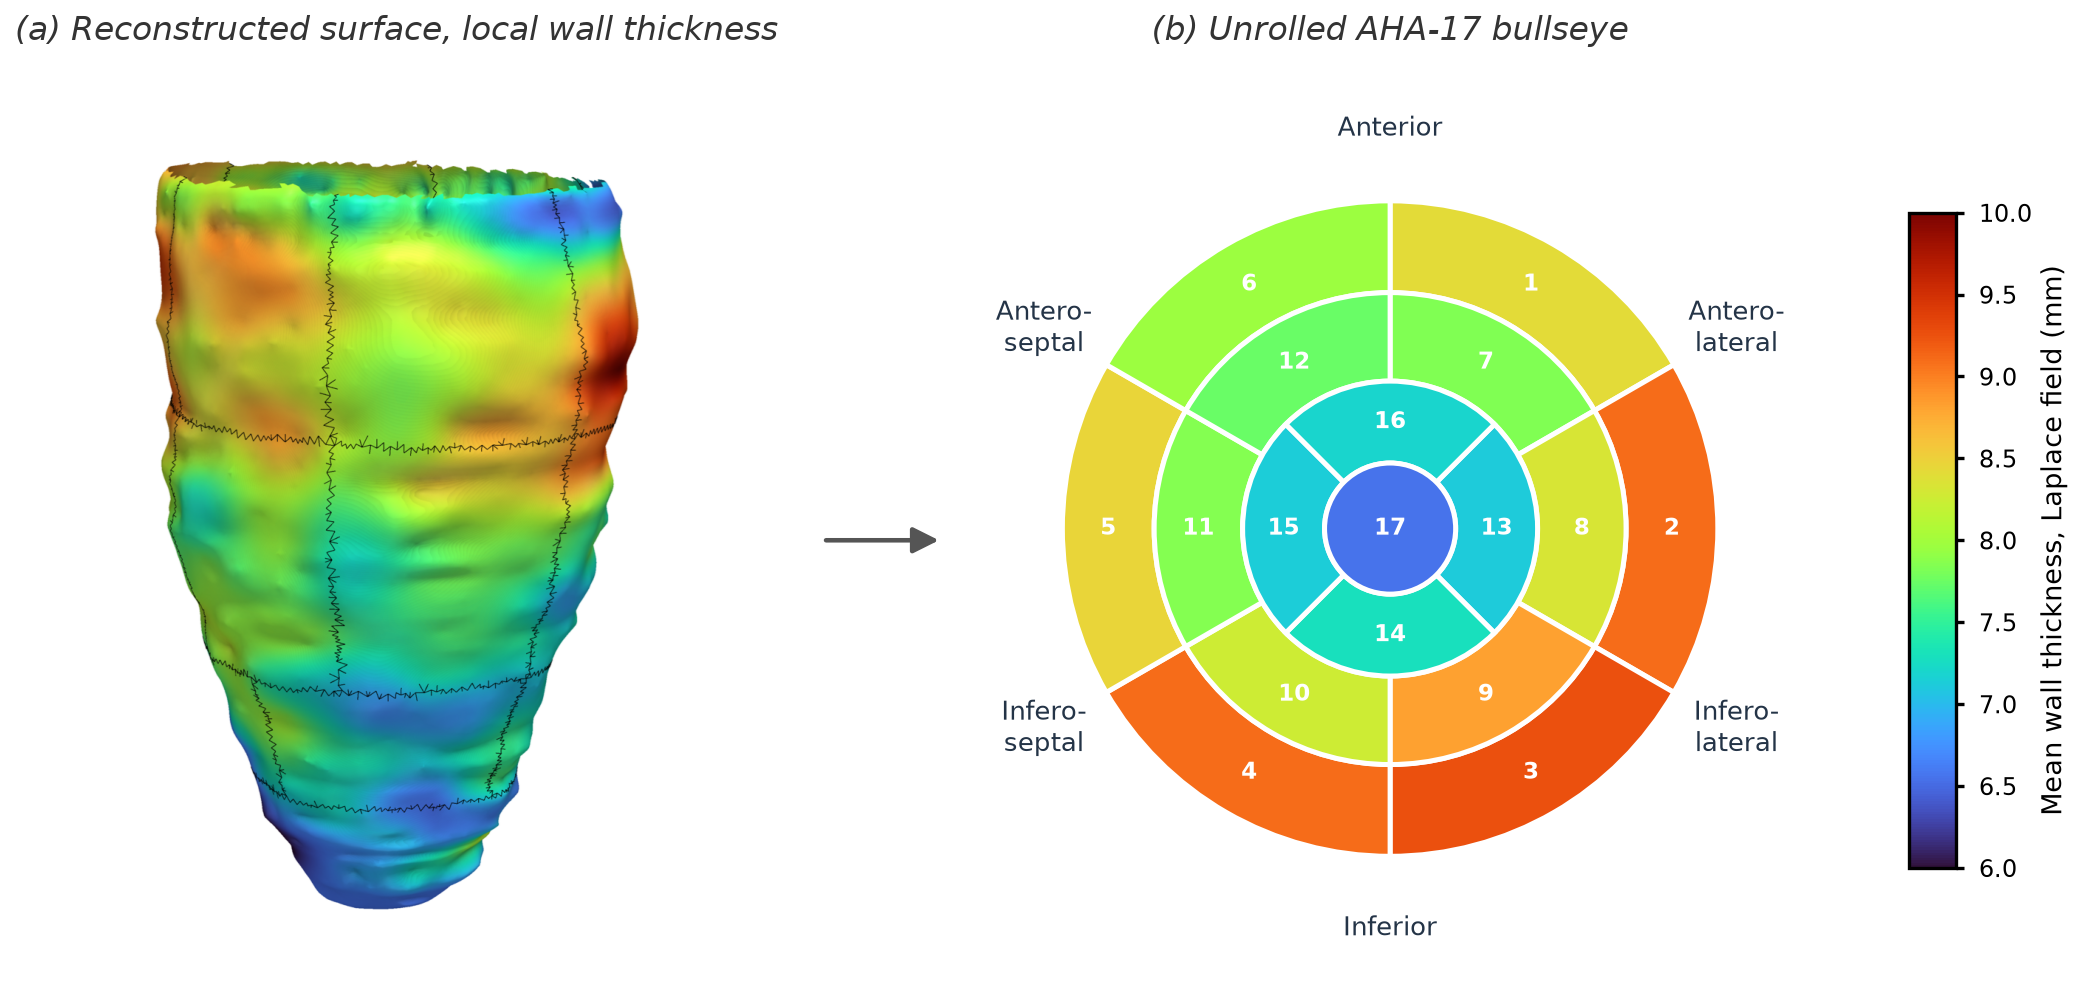
\includegraphics[width=\textwidth]{results_recon_aha17}
  \caption[AHA 17-segment wall-thickness analysis]    {AHA 17-segment analysis of the
      representative case at ED: (a) reconstructed surface coloured by the mean
      Laplace-field wall thickness of each segment; (b) the same values on the
      standard bullseye, with basal (1--6), mid-cavity (7--12) and apical
      (13--16) rings and the apical cap (17).}
  \label{fig:aha17-bullseye}
\end{figure}

\Cref{fig:aha17-bullseye} shows the partition on the representative case, with
each patch coloured by its mean thickness in panel~(a) and the same means
unrolled onto the standard bullseye in panel~(b), basal ring outermost and
apical cap at the centre.

\Cref{tab:aha17-cohort} reports the
regional pattern over the 30-patient ACDC pathology subset and its change
between phases. Entries are segment means averaged across patients; variation
between patients is examined in~\cref{tab:aha17-group-effects}.

Over the ACDC pathology subset the reconstructed wall averages 9.21~mm at ED
and 13.87~mm at ES, corresponding to 50.6\% relative thickening. At ED the
septal mid-cavity segments are the thickest, while the apical cap is the
thinnest at 7.76~mm. Every segment thickens between phases; the smallest
relative change is 32.1\% in the basal anteroseptal segment and the largest
is 64.6\% in the mid inferolateral segment. No fitting baseline is available
at ES, so these phase values describe the model output only.

\begin{table}[H]
  \centering
  \caption[AHA 17-segment thickness over the ACDC pathology subset]{Regional AHA
    17-segment wall thickness on the reconstructed geometry over the
    30-patient ACDC pathology subset.}
  \label{tab:aha17-cohort}
  \thesistablestyle
  \begin{tabular*}{\textwidth}{@{\extracolsep{\fill}}r l r r r@{}}
    \toprule
    \multicolumn{1}{c}{\textbf{\#}} & \textbf{Segment}
      & \multicolumn{1}{c}{\textbf{ED (mm)}} & \multicolumn{1}{c}{\textbf{ES (mm)}}
      & \multicolumn{1}{c}{\textbf{$\Delta$ (\%)}} \\
    \midrule
    1  & Basal anterior       &  9.99 & 13.71 & +37.1 \\
    2  & Basal anteroseptal   & 10.15 & 13.40 & +32.1 \\
    3  & Basal inferoseptal   &  9.89 & 13.43 & +35.7 \\
    4  & Basal inferior       &  9.09 & 13.81 & +51.9 \\
    5  & Basal inferolateral  &  8.93 & 14.27 & +59.8 \\
    6  & Basal anterolateral  &  9.53 & 13.87 & +45.5 \\
    \addlinespace
    7  & Mid anterior         &  9.19 & 13.79 & +50.0 \\
    8  & Mid anteroseptal     & 10.37 & 14.68 & +41.6 \\
    9  & Mid inferoseptal     & 10.19 & 15.05 & +47.6 \\
    10 & Mid inferior         &  9.25 & 14.41 & +55.8 \\
    11 & Mid inferolateral    &  9.09 & 14.96 & +64.6 \\
    12 & Mid anterolateral    &  8.99 & 14.17 & +57.6 \\
    \addlinespace
    13 & Apical anterior      &  8.50 & 13.63 & +60.3 \\
    14 & Apical septal        &  8.77 & 13.86 & +58.1 \\
    15 & Apical inferior      &  8.44 & 13.29 & +57.5 \\
    16 & Apical lateral       &  8.43 & 13.78 & +63.6 \\
    \addlinespace
    17 & Apex                 &  7.76 & 11.69 & +50.7 \\
    \midrule
    \multicolumn{2}{@{}l}{\textbf{Overall}} & \textbf{9.21} & \textbf{13.87}
      & \textbf{+50.6} \\
    \bottomrule
  \end{tabular*}
  \vspace{0.8em}

  \begin{minipage}{\textwidth}
    \footnotesize\singlespacing
    \textit{Note.} Values are means for the 30 ACDC test patients used in the
    pathology analysis, measured with the Laplace field. $\Delta$ is the relative
    thickening from ED to ES.
  \end{minipage}
\end{table}

\Cref{tab:aha17-thickening} separates the normal and HCM patients, and both
groups show an internally coherent regional pattern. In the normal cases the ED thickness varies little around the base and the
mid-cavity, from 7.92 to 8.81~mm, and tapers towards the apex, where the
apical cap at 6.80~mm is the thinnest region. Every segment thickens from
ED to ES, and the thickening is graded along the long axis:
the apical segments thicken by 52\% to 64\%, the mid-cavity segments by
51\% to 64\% and the basal segments by 37\% to 61\%. Over the normal
group the mean thickness rises from 7.99~mm to 12.21~mm, a thickening of
52.9\%.

\begin{table}[H]
  \centering
  \caption[AHA 17-segment thickness: NOR versus HCM]{Regional AHA 17-segment wall thickness on the reconstructed geometry for
    the normal and HCM groups.}
  \label{tab:aha17-thickening}
  \thesistablestyle
  \begin{tabular*}{\textwidth}{@{\extracolsep{\fill}}r l r r r r r r@{}}
    \toprule
    & & \multicolumn{3}{c}{\textbf{Normal (NOR, $n=20$)}}
      & \multicolumn{3}{c}{\textbf{Hypertrophic (HCM, $n=10$)}} \\
    \cmidrule(lr){3-5} \cmidrule(lr){6-8}
    \multicolumn{1}{c}{\textbf{\#}} & \textbf{Segment}
      & \multicolumn{1}{c}{\textbf{ED}} & \multicolumn{1}{c}{\textbf{ES}} & \multicolumn{1}{c}{\textbf{$\Delta$}}
      & \multicolumn{1}{c}{\textbf{ED}} & \multicolumn{1}{c}{\textbf{ES}} & \multicolumn{1}{c}{\textbf{$\Delta$}} \\
    & & \multicolumn{2}{c}{\textbf{(mm)}} & \multicolumn{1}{c}{\textbf{(\%)}}
      & \multicolumn{2}{c}{\textbf{(mm)}} & \multicolumn{1}{c}{\textbf{(\%)}} \\
    \midrule
    1  & Basal anterior       &  8.72 & 12.25 & +40.4 & 12.54 & 16.62 & +32.6 \\
    2  & Basal anteroseptal   &  8.81 & 12.10 & +37.4 & 12.83 & 16.02 & +24.9 \\
    3  & Basal inferoseptal   &  8.68 & 11.96 & +37.8 & 12.32 & 16.35 & +32.8 \\
    4  & Basal inferior       &  8.16 & 12.53 & +53.6 & 10.96 & 16.37 & +49.4 \\
    5  & Basal inferolateral  &  7.94 & 12.81 & +61.3 & 10.91 & 17.19 & +57.5 \\
    6  & Basal anterolateral  &  8.38 & 12.12 & +44.6 & 11.83 & 17.37 & +46.9 \\
    \addlinespace
    7  & Mid anterior         &  7.94 & 12.10 & +52.5 & 11.70 & 17.16 & +46.6 \\
    8  & Mid anteroseptal     &  8.55 & 12.98 & +51.7 & 13.99 & 18.10 & +29.4 \\
    9  & Mid inferoseptal     &  8.57 & 12.98 & +51.4 & 13.43 & 19.17 & +42.8 \\
    10 & Mid inferior         &  7.93 & 12.46 & +57.1 & 11.89 & 18.32 & +54.1 \\
    11 & Mid inferolateral    &  7.96 & 13.02 & +63.5 & 11.35 & 18.84 & +66.0 \\
    12 & Mid anterolateral    &  7.92 & 12.39 & +56.4 & 11.13 & 17.73 & +59.3 \\
    \addlinespace
    13 & Apical anterior      &  7.28 & 11.75 & +61.4 & 10.96 & 17.40 & +58.7 \\
    14 & Apical septal        &  7.49 & 12.00 & +60.2 & 11.33 & 17.59 & +55.3 \\
    15 & Apical inferior      &  7.28 & 11.72 & +61.1 & 10.76 & 16.43 & +52.6 \\
    16 & Apical lateral       &  7.33 & 12.03 & +64.0 & 10.61 & 17.28 & +62.9 \\
    \addlinespace
    17 & Apex                 &  6.80 & 10.32 & +51.8 &  9.67 & 14.71 & +52.1 \\
    \midrule
    \multicolumn{2}{@{}l}{\textbf{Overall}} & \textbf{7.99} & \textbf{12.21} & \textbf{+52.9}
      & \textbf{11.68} & \textbf{17.23} & \textbf{+47.5} \\
    \bottomrule
  \end{tabular*}
  \vspace{0.8em}

  \begin{minipage}{0.92\textwidth}
    \footnotesize\singlespacing
    \textit{Note.} Values are group means measured with the     Laplace field. $\Delta$ is the
        relative thickening from ED to ES. These measurements summarise the model
    output reconstructed from sparse SAX contours and are not an independent
    anatomical reference.
  \end{minipage}
\end{table}
 
HCM thickness exceeds NOR thickness in every segment, with the largest differences
in the mid-cavity anteroseptal and inferoseptal segments, where the HCM group
reaches 13.99 and 13.43~mm compared with 8.55 and 8.57~mm in the normal
group. \Cref{tab:aha17-group-effects} evaluates this separation at the patient
level rather than treating the segments as independent observations. Each
patient contributes one value per outcome: the mean and the largest of the ED
segment means, and the relative ED-to-ES increase, so group differences in
thickening are in percentage points. The confidence intervals come from
resampling patients within each group~\parencite{efron1979bootstrap}, and
Hedges' $g$~\parencite{hedges1981effectsize} expresses the group difference
relative to the patient-to-patient spread.

\begin{table}[H]
  \centering
  \caption[Patient-level NOR--HCM wall-thickness differences]  {Patient-level comparisons between the
      normal and HCM groups (mean~\textpm{} SD). Differences are HCM minus NOR with
      95\% percentile-bootstrap CIs from 10\,000 resamples~\parencite{efron1979bootstrap}; positive Hedges' $g$~\parencite{hedges1981effectsize} indicates a larger HCM value. Bold CIs
      exclude zero.}
  \label{tab:aha17-group-effects}
  \thesistablestyle
  \begin{tabular*}{\textwidth}{@{\extracolsep{\fill}}l c c c c@{}}
    \toprule
    \textbf{Measure} & \textbf{NOR} & \textbf{HCM}
      & \textbf{Difference (95\% CI)} & \textbf{Hedges' $g$} \\
    \midrule
    Mean ED AHA-17 thickness (mm)
      & 7.99~\textpm{} 0.88 & 11.66~\textpm{} 1.66 & \textbf{+3.67 [2.54, 4.67]} & 3.01 \\
    Maximum ED segment (mm)
      & 9.07~\textpm{} 0.98 & 14.44~\textpm{} 1.94 & \textbf{+5.37 [4.11, 6.56]} & 3.82 \\
    Systolic thickening (percentage points)
      & 53.2~\textpm{} 11.6 & 47.9~\textpm{} 11.5 & \textminus{}5.3 [\textminus{}13.9, 3.0] & \textminus{}0.45 \\
    \bottomrule
  \end{tabular*}
\end{table}

Both ED confidence intervals exclude zero, and both effect sizes are large. The
interval for relative systolic thickening includes zero, so this cohort shows
no clear group difference in proportional thickening. None of the normal cases
and three of the ten HCM cases have a maximum segment mean above the 15~mm
clinical reference line~\parencite{ommen2020hcm}.

\Cref{fig:group-thickness-distributions} shows the patient-level distributions
of absolute ED thickness and relative systolic thickening.

\begin{figure}[H]
  \centering
  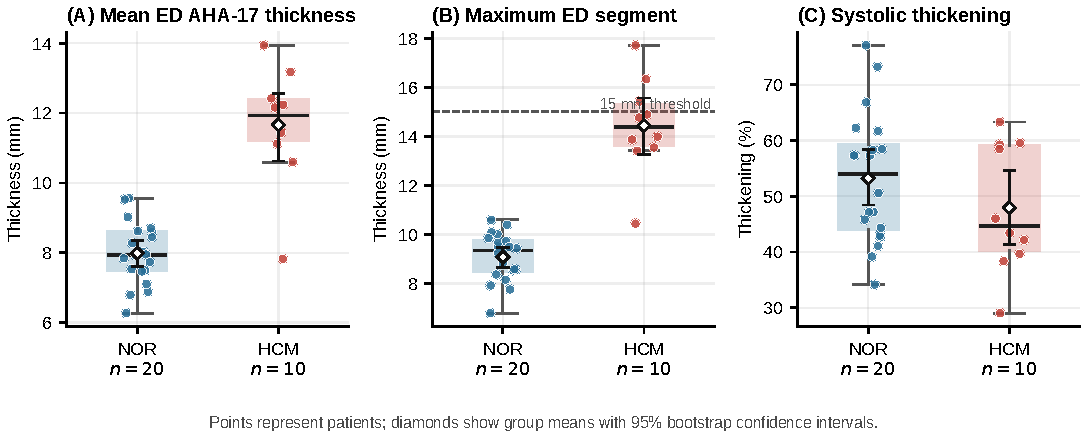
\includegraphics[width=\textwidth]{results_group_thickness_distributions}
  \caption[Patient-level NOR--HCM wall-thickness outcomes]  {Patient-level AHA-17 wall-thickness
      outcomes for the normal and HCM groups. The dashed line marks the 15~mm
      clinical reference for maximal ED LV wall thickness; the plotted maximum
      segment mean is not diagnostically equivalent to it.}
  \label{fig:group-thickness-distributions}
\end{figure}

The two groups overlap more in relative thickening than in absolute thickness.
\FloatBarrier

\section{Discussion}
\label{sec:discussion}
\noindent
The results are interpreted below against the three research questions of~\cref{sec:research-questions}. Because no independent 3D reference is available~(\cref{sec:setup}), each answer concerns fidelity to the input contours,
agreement between methods, or internal consistency, not anatomical accuracy.

\textbf{RQ1} compares the learned reconstruction with RBF and SSM
reconstructions of the same contours. Closure does not separate the methods:
every surface is watertight after the shared repair stage, so closure is a
property of the pipeline rather than of the learned prior. The methods differ
instead in how closely they follow the contours and in the geometry they infer
between slices.

The model follows its input rings to within about one in-plane pixel~(\cref{tab:contour-fidelity}). Exact agreement with the rings is not the aim.
Expert contours contain annotation errors and are restricted to the pixel grid,
so a surface that matches them to 0.13~mm, as the RBF fit does by
construction, also reproduces those errors. A consistent deviation of about one
pixel is compatible with a surface that smooths this noise rather than one that
misses the observations. The SSM fit has a similar mean distance but a much
wider spread between patients, and the pathology subset locates the source of
that spread: the SSM distance increases markedly on HCM cases, whereas the model
distance changes little. A population model can represent only shapes within
the variation of its training population, and thick hypertrophic walls lie
partly outside it. The model, which is conditioned directly on the contours,
appears less tied to an average shape.

The pairwise comparison shows where the three reconstructions disagree~(\cref{tab:reconstruction-agreement}). On the endocardium they differ by about
one in-plane pixel, far less than the 10~mm slice spacing, and cavity DSC is
high for every pair. Myocardial agreement is clearly lower, and myocardial
volume varies by several tens of millilitres between methods. The cause lies in
what the data constrain. The contours fix the cavity outline at each slice, but
both surfaces must be inferred between slices, and small changes in the
inferred epicardium alter myocardial volume and thickness much more than cavity
overlap. Lower myocardial agreement therefore shows that the wall geometry
depends on the reconstruction prior; it does not show that one method is
anatomically better. Because wall thickness is measured on this geometry, the
spread between methods is a lower bound on the uncertainty of every thickness
value in this chapter, and selecting one method as correct would not remove it.
The model lies closest to the RBF fit, but part of this agreement is expected,
because the training targets were produced by a similar surface fit~(\cref{subsec:baselines}).

Slice removal degrades the three methods by similar amounts~(\cref{tab:slice-degradation}). The model has the largest epicardial
displacement with three slices but not the largest change in myocardial volume,
so no method is more robust on every metric. These values describe stability
relative to each method's own complete-stack surface, not anatomical error.

\textbf{RQ2} asks whether one phase-conditioned model can reconstruct paired
surfaces at ED and ES while keeping a positive wall thickness. The architecture
fixes the order of the two surfaces, because the epicardial field is defined as
the endocardial field minus a strictly positive offset. On the output, the
Laplace-derived thickness increases in all seventeen AHA segments between ED and
ES~(\cref{tab:aha17-cohort}), which is the expected direction of systolic wall
thickening. The evaluation did not measure the minimum pointwise separation
between the extracted meshes, test for surface intersections after repair, or
report the ED--ES change in cavity volume, and no fitting baseline is available
at ES. The evidence therefore supports a phase-dependent reconstruction with a
thickening wall. Positive separation holds in the continuous fields by
construction, but it has not been verified at every point of the extracted
meshes, and accuracy at ES remains untested.

\textbf{RQ3} asks how wall thickness depends on the reconstruction prior and on
the measurement method, and whether regional and pathology-related differences
are retained. Both factors change the measured thickness, in different ways.

With the method fixed, the reconstruction prior mainly shifts the absolute
scale~(\cref{tab:wall-thickness-geometry-agreement}). Thickness on the model and
on the RBF fit is almost perfectly correlated across patients, yet the model is
consistently thicker: the RBF fit preserves the ranking of patients but changes
their absolute values. The SSM fit changes both the scale and, to a lesser
extent, the ranking, as expected from a stronger shape prior. A high correlation
therefore does not imply agreement in millimetres; only the bias reveals the
offset.

With the geometry fixed, the measurement path matters~(\cref{tab:wall-thickness-agreement}). Yezzi--Prince and the EDT boundary sum
agree closely with the Laplace field, whereas the SDF cone-ray method is both
biased and highly variable. The most likely cause is geometric. A straight ray
leaves the myocardium too early or too late wherever the wall curves, whereas
the Laplace and Yezzi--Prince paths follow the curvature of the wall and the
EDT boundary sum does not depend on a single direction. The two effects are of
similar size: the cone-ray bias of +3.31~mm is close to the 2.53 to
2.91~mm offset between the model and SSM geometries with the non-ray methods.
Thickness values are therefore comparable only when both the reconstruction and
the measurement method are the same.

For the second part of RQ3, the reconstruction retains differences between
patient groups instead of reproducing an average shape. At the patient level,
the HCM group is thicker at ED in both mean thickness and thickest segment, with
confidence intervals that exclude zero and large effect sizes~(\cref{tab:aha17-group-effects}). Relative systolic thickening does not
separate the groups in this cohort. With ten HCM patients, these are
descriptive differences within the model output rather than evidence of
diagnostic ability.

\section{Limitations of the Evaluation}
\label{sec:threats}
\noindent
The central limitation concerns the reference: no public dataset provides
independently acquired 3D ground-truth surfaces for these scans, so the
reconstruction is evaluated through fidelity to the observed contour rings and
agreement with alternative reconstructions of those rings. The pairwise
Chamfer distances measure disagreement between reconstruction priors,
not distance from true anatomy. The same caveat applies to the wall-thickness
comparison: the input is a stack of contours separated by several millimetres,
so no method used in this chapter carries measured through-plane information,
and the way that gap is inferred shifts the measured thickness. Absolute
millimetre values should not be over-interpreted; the comparisons
that the data support are relative ones between pipelines evaluated on identical
input. The wall-thickness study compares methods and how consistently they measure
thickness; it does not validate clinical use. Without expert manual wall-thickness measurements,
this work can claim an objective and locally resolved computational framework,
but cannot establish that it can replace clinical measurement methods.

Several further factors limit how widely these results can be applied, and the whole
evaluation should be read as preliminary. The general evaluation uses held-out
patients from ACDC and M\&Ms-2, whereas the regional analysis by disease group
is limited to 30 ACDC test patients: 20 normal and 10 with
HCM. This subset is far too small to support claims of
clinical or pathological generalisation, and the HCM subgroup in
particular can only suggest a pattern rather than support broad conclusions. The regional
analysis carries a further dependency: each patient contributes seventeen
segments, so the segment values are repeated measures within a patient rather
than independent samples, and they are reported as a descriptive summary for
that reason. The relative thickening
figures deserve particular caution, because dividing a systolic by a diastolic
thickness amplifies small differences in where the wall is sampled. The
regional summaries also depend on the AHA orientation, while all mesh-based
measurements depend on the inference grid. A finer grid or an alternative
anatomical frame could shift the values. Only the heatmap in~\cref{fig:recon-thickness-3d} is scaled to the input segmentation; the tables
report thickness measured directly on the meshes. The
reconstruction additionally inherits the
quality of the input segmentation, and the training data span more than one
collection, so some differences between the acquisition sources are expected.
Finally, the synthetic epicardium used during pre-training is constructed
rather than measured. Fine-tuning on clinical data is intended to correct for
this difference, but the synthetic shapes may still influence the output. A
larger cohort, and ideally a dataset with genuine 3D ground truth, would be
needed to confirm the results reported here.

Reconstruction comparisons are bounded in the same way. The implicit
fit and the SSM fit were chosen because their priors differ from each
other and from the learned one, so the spread between the three bounds the
influence of the prior; it does not identify which is closest to the anatomy.
Contour fidelity cannot settle the question either, because it evaluates
only the observed rings and not the geometry between them.
The slice-removal criterion in~\cref{tab:slice-degradation} may favour a
stable prior that responds weakly to the observations as much as a method that
generalises well from them. Because the acquired stacks vary in length, the
three slice-removal levels are also supported by different subsets of patients,
and the most extensive removal level rests on the longest stacks alone.
The comparison does not cover spline lofting, Poisson reconstruction, or other
learned models. No controlled experiment tests the effect of removing
synthetic pre-training, local conditioning, phase conditioning, or positive
surface coupling. The
comparison describes the model alongside two conventional alternatives, but
cannot show which component produced its behaviour or whether the full
architecture is necessary.
